This paper is for the purposes of teaching the basics of graphing lines and planes in 3D space; Providing knowledge on how to determine properties of equations or certain functions. Graphs will be rendered using two software tools code and resources will be provided to use:
\begin{itemize}
\item{Python - (Matplotlib library)}
\item{Geogebra - (Online Web Platform)}
\end{itemize}

Consider the following graph:
\begin{figure}[htb]
\centering
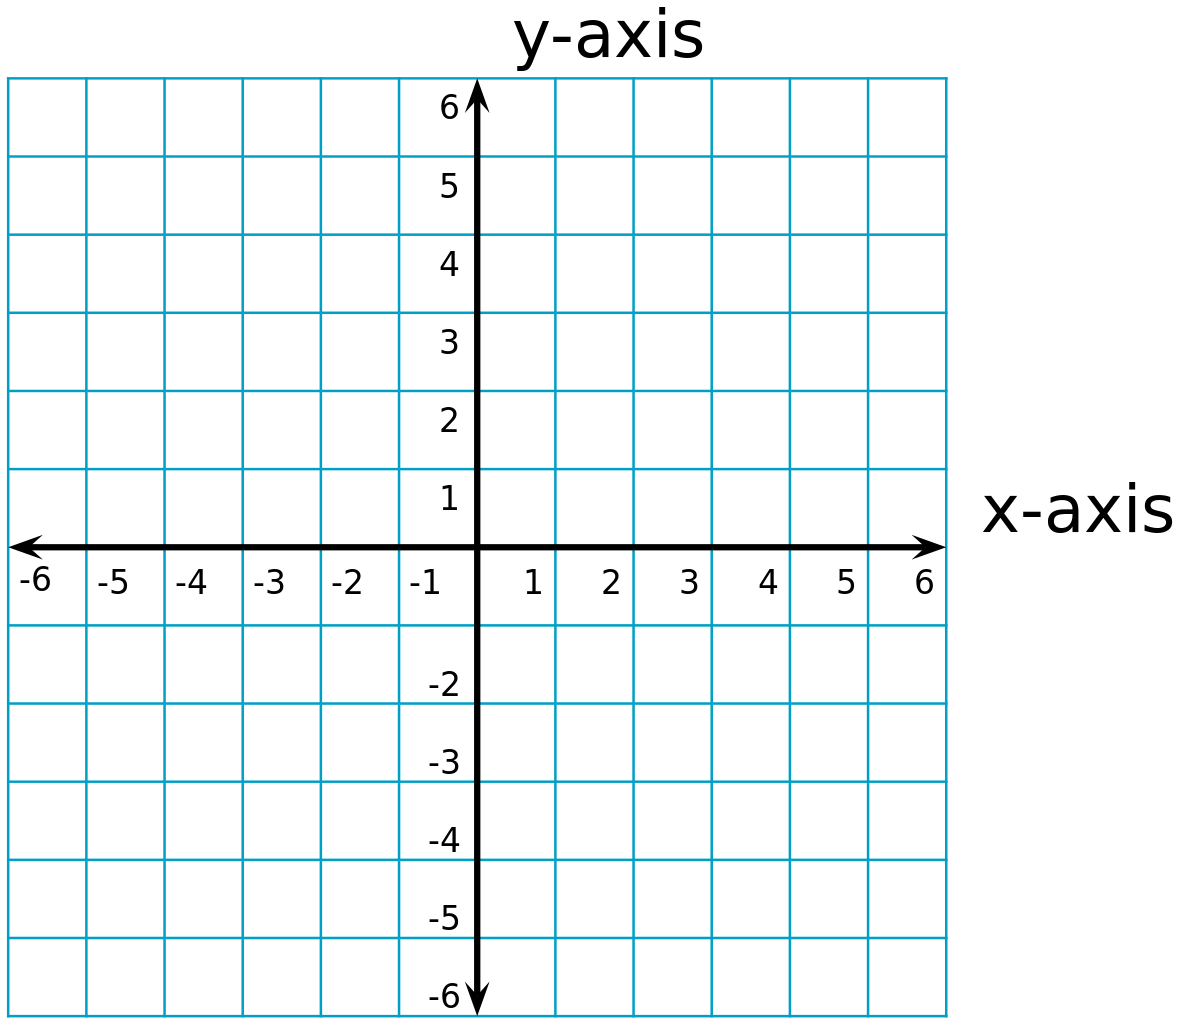
\includegraphics[width=0.4\textwidth]{fig1.png}
\caption{Cartesian 2D Graph}
\label{fig:line}
\end{figure}

Remember that this graph is a function of x and y (which we are all used to). But now we want to graph this function in 3D space as well. A new z-axis is needed.

Thus, our 3D Space canvas will look like this:
\begin{figure}[htb]
\centering
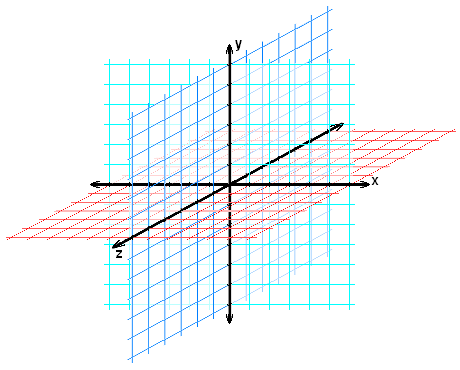
\includegraphics[width=0.4\textwidth]{fig2.png}
\caption{Cartesian 3D Graph}
\label{fig:line3d}
\end{figure}

Motivation for this paper is that there is some lacking of information for 3D planes in 3D space/not enough notes compiled in a simple way to understand. Since 3D planes content is in my first year University content, I will use this to refer back to in the future for Linear Algebra but lets also have fun exploring software to plot 3D graphs/functions outside my University content.
We will now play and explore the 3D world and space mathematically. Hope you enjoy!
